\documentclass[tikz,border=5pt]{standalone}
\pdfinfoomitdate=1
\pdftrailerid{}
\pdfsuppressptexinfo=-1
\usepackage{pgfplots}
\usepgfplotslibrary{groupplots}
\pgfplotsset{compat=1.18}
\pgfplotsset{colormap/viridis}
\definecolor{atlas0}{HTML}{0072B2}
\definecolor{atlas1}{HTML}{D55E00}
\definecolor{atlas2}{HTML}{009E73}
\definecolor{atlas3}{HTML}{E69F00}
\definecolor{atlas4}{HTML}{56B4E9}
\definecolor{atlas5}{HTML}{CC79A7}
\definecolor{atlas6}{HTML}{000000}
\definecolor{atlas7}{HTML}{F0E442}
% NATO SERS figure F40; data_sha256=949803bbf84ddfb965db8282260d16a71432b340a43874a1a92e44746690e8c3
% caption=(S) RQ-P01 paired aggregation diagnostic for C09. Each point is one held-domain × split-repeat endpoint; x is spectrum balanced accuracy and y is instrument-balanced physical-master balanced accuracy from identical outer predictions. The diagonal is equality. Unavailable pairs remain in the frozen table but have no fabricated coordinates. Repeats are technical and domains, not spectra, define the comparison units.
\begin{document}
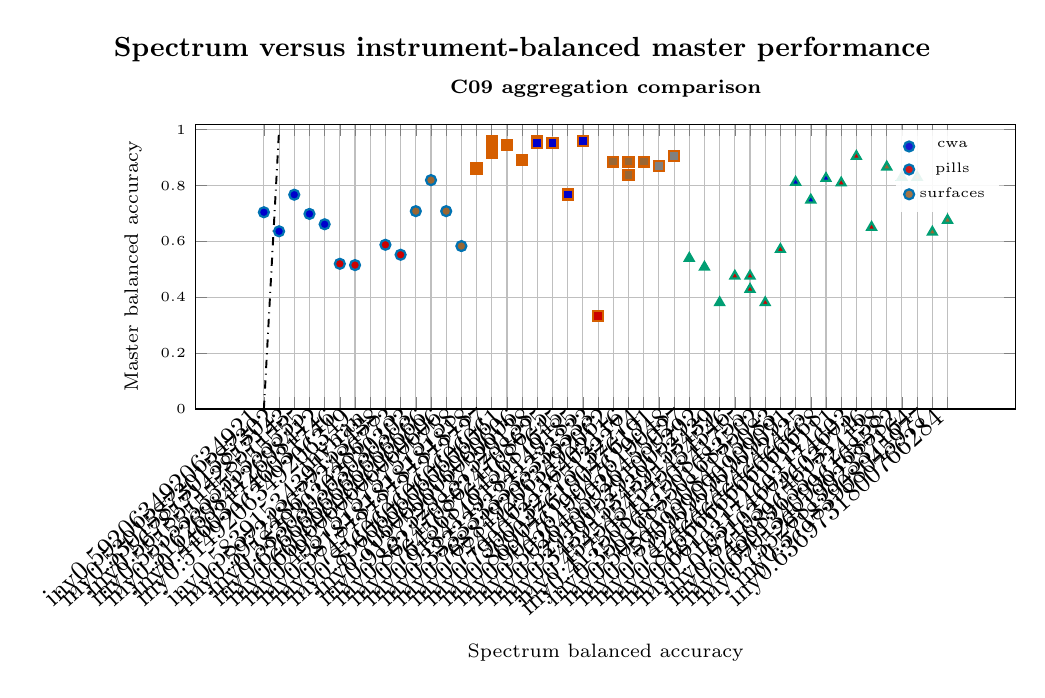
\begin{tikzpicture}
\begin{groupplot}[group style={group size=1 by 1, horizontal sep=1.35cm, vertical sep=1.5cm}, width=12.00cm, height=5.2cm, grid=major, tick label style={font=\tiny}, label style={font=\scriptsize}, title style={font=\scriptsize\bfseries,align=center}, legend style={font=\tiny,draw=none,fill=white,fill opacity=0.9,text opacity=1}]
\nextgroupplot[title={C09 aggregation comparison},xlabel={Spectrum balanced accuracy},ylabel={Master balanced accuracy},ymin=0,ymax=1.02,xtick={0,1,2,3,4,5,6,7,8,9,10,11,12,13,14,15,16,17,18,19,20,21,22,23,24,25,26,27,28,29,30,31,32,33,34,35,36,37,38,39,40,41,42,43,44,45},xticklabels={0.5920634920634921,0.5301587301587302,0.567857142857143,0.5555555555555555,0.5162698412698412,0.446031746031746,0.5149206349206349,nan,0.5839153439153438,0.5972486772486773,0.583030303030303,0.6266666666666666,0.6606060606060606,0.4957575757575758,0.5818181818181818,0.7477272727272727,0.8560606060606061,0.706060606060606,0.9137529137529138,0.8624708624708625,0.7645687645687645,0.9184149184149185,0.3333333333333333,0.7688492063492062,0.7741402116402116,0.7900132275132274,0.8690476190476191,0.9047619047619048,0.5026455026455027,0.5291005291005292,0.3439153439153439,0.4545454545454546,0.41750841750841755,0.3501683501683502,0.5084175084175083,0.7590909090909091,0.7424242424242425,0.8166666666666668,0.6611111111111111,0.7103174603174603,0.621031746031746,0.7456896551724138,0.6901340996168582,0.7552681992337164,0.57183908045977,0.6369731800766284},x tick label style={rotate=42,anchor=east,font=	iny}]
\addplot+[color=atlas0,mark=*,mark size=1.8pt,line width=0.8pt,only marks] coordinates {(0,0.70436508) (1,0.63624339) (2,0.76719577) (3,0.6984127) (4,0.66137566)};
\addlegendentry{cwa}
\addplot+[color=atlas0,mark=*,mark size=1.8pt,line width=0.8pt,only marks] coordinates {(5,0.51984127) (6,0.51521164) (8,0.58796296) (9,0.55224868)};
\addplot+[color=atlas0,mark=*,mark size=1.8pt,line width=0.8pt,only marks] coordinates {(10,0.70833333) (11,0.81944444) (12,0.70833333) (13,0.58333333)};
\addplot+[color=atlas1,mark=square*,mark size=1.8pt,line width=0.8pt,only marks] coordinates {(14,0.86111111) (15,0.91666667) (15,0.95833333) (16,0.94444444) (17,0.89166667)};
\addlegendentry{pills}
\addplot+[color=atlas1,mark=square*,mark size=1.8pt,line width=0.8pt,only marks] coordinates {(18,0.95833333) (18,0.95238095) (19,0.95238095) (20,0.76785714) (21,0.95833333)};
\addplot+[color=atlas1,mark=square*,mark size=1.8pt,line width=0.8pt,only marks] coordinates {(22,0.33333333) (22,0.33333333) (22,0.33333333) (22,0.33333333) (22,0.33333333)};
\addplot+[color=atlas1,mark=square*,mark size=1.8pt,line width=0.8pt,only marks] coordinates {(23,0.88571429) (24,0.83809524) (24,0.88571429) (24,0.83809524) (25,0.88571429)};
\addplot+[color=atlas1,mark=square*,mark size=1.8pt,line width=0.8pt,only marks] coordinates {(26,0.86904762) (26,0.86904762) (26,0.86904762) (26,0.86904762) (27,0.9047619)};
\addplot+[color=atlas2,mark=triangle*,mark size=1.8pt,line width=0.8pt,only marks] coordinates {(28,0.53968254) (29,0.50793651) (30,0.38095238)};
\addlegendentry{surfaces}
\addplot+[color=atlas2,mark=triangle*,mark size=1.8pt,line width=0.8pt,only marks] coordinates {(31,0.47619048) (32,0.42857143) (32,0.47619048) (33,0.38095238) (34,0.57142857)};
\addplot+[color=atlas2,mark=triangle*,mark size=1.8pt,line width=0.8pt,only marks] coordinates {(35,0.81212121) (36,0.74848485) (37,0.82575758)};
\addplot+[color=atlas2,mark=triangle*,mark size=1.8pt,line width=0.8pt,only marks] coordinates {(38,0.80952381) (39,0.9047619) (40,0.65079365)};
\addplot+[color=atlas2,mark=triangle*,mark size=1.8pt,line width=0.8pt,only marks] coordinates {(41,0.86666667) (42,0.82962963) (43,0.82962963) (44,0.63333333) (45,0.67592593)};
\addplot[black,dashdotted,line width=0.7pt,forget plot] coordinates {(0,0) (1,1)};
\end{groupplot}
\node[font=\normalsize\bfseries,anchor=south] at (current bounding box.north) {Spectrum versus instrument-balanced master performance};
\end{tikzpicture}
\end{document}
